%%
%% If you intend to use figures of formats jpg, png or pdf and want the
%% output to be immediately a pdf file, compile with pdflatex.
%%
%% If you want to use eps or ps figures, your output will be a dvi
%% file that can be converted to ps and pdf formats. In this case you
%% should compile your document with latex.
%%
%%This template is compatible with both methods.
%%
\title{{\normalsize Optimization and Algorithms} \\
Financial Portfolio Optimization}
\author{
        Bernardo Gomes
        \and
        Kishan Rama
        \and
        Tom\'as Falcato \\ {\tt bernardo.n.gomes@ist.utl.pt} \and {\tt kishan.rama@ist.utl.pt} \and {\tt tomas.falcato.costa@ist.utl.pt} \\
        Instituto Superior T\'{e}cnico}
\date{\today}


\documentclass[a4paper]{IEEEtran}
\usepackage[utf8]{inputenc}
\usepackage{graphicx}
\usepackage{amsmath}
\usepackage{amsfonts}
\usepackage{listings}
\usepackage{algorithmic}
\usepackage{subfig}

\begin{document}
\maketitle

\begin{abstract}
 Para o problema de \textit{Financial portfolio optimization}, dado um conjunto de \textit{assets}, pretende-se obter uma forma de distribuir o dinheiro a investir por forma a maximizar o retorno. A cada \textit{asset}, existe um risco associado, sendo que o risco de cada um poderá, ou não, influenciar o risco dos restantes.
%----------------------------------------------------------------------------------------------------------------
%PERGUNTAR!!!!!!!!!!!!!!!!!!!!!!!!!!!!!!!!!!!
Se considerarmos todas as variáveis inerentes à otimização deste tipo de problemas, iremos obter funções não convexas, pelo que se considera uma aproximação facilmente computável através de otimização convexa e cujos resultados, obtidos a partir do \textit{software CVX}, são bastante próximos dos ótimos. 
%----------------------------------------------------------------------------------------------------------------
%segunda parte do projeto
Posteriormente, o problema foi reformulado por forma a obter uma solução sub-ótima mas com menor tempo de computação. 
%----------------------------------------------------------------------------------------------------------------
%principais resultados
%PERGUNTAR!!!!!!!!!!!!!!!!!!!!!!!!!!!!!!!!!!!!!!!!!!!!!
%----------------------------------------------------------------------------------------------------------------
\end{abstract}

\smallskip
\noindent \textbf{Keywords.} Portfolio Optimization \textbullet CVX \textbullet Barrier Method \textbullet Newton Method

\section{Introdução}
\label{sec:introduction}
Este artigo pretende obter uma solução para o problema de \textit{Portfolio Optimization}. Para tal, a nossa abordagem maximiza o retorno esperado e minimiza o risco de investimento tendo em conta a aversão ao risco colocada pela pessoa que investe.

Na vida real, o problema discutido neste artigo tem extrema importância na medida em que praticamente todas as pessoas fazem investimentos do seu dinheiro. A formulação terá em conta não só os casos em que a pessoa pretende rápidos retornos e pretende que estes sejam bastante elevados, independentemente de o risco a ele associado ser relativamente elevado, como também casos cujo objetivo seja obter um resultado de longo prazo em que a aversão ao risco é um fator preponderante face à quantia recebida.

%contributions!!!!!!!!!!!!
Por forma a resolver, e melhor compreender o problema, numa primeira abordagem foi utilizado o \textit{software CVX}. Posteriormente, implementa-se a mesma resolução do problema, mas com este reescrito por forma a utilizar o algoritmo \textit{Barrier Method}. 


O artigo está organizado da forma enunciada de seguida. No capítulo
~\ref{sec:problem-formulation}, é introduzida a função a otimizar e as respetivas variáveis,  capítulo~\ref{sec:cvx} descreve a abordagem para a utilização do \textit{software CVX}, sendo esta alterada para a utilização do \textit{Barrier Method}, descrito no capítulo~\ref{sec:barrier-method}. Os resultados obtidos nas duas fases são discutidos e comparados em~\ref{sec:numerical-results}. As conclusões são apresentadas posteriormente em ~\ref{sec:conclusion}.

\section{Formulação do Problema}
\label{sec:problem-formulation}

Para a obtenção dos resultados do problema descrito anteriormente, a função utilizada foi a seguinte:
\begin{equation}
  \label{eq:problem}
\begin{array}[t]{ll} \text{maximize} & \mu^\top \omega - \gamma \omega^\top \Sigma \omega \\
\text{subject to} & 1^\top \omega = 1 \\ &  \omega \in \mathbb{R}_+^n \end{array}
\end{equation}

Apresenta-se de seguida a descrição das variáveis da função de otimização:

\begin{itemize}
\item  $\omega$ $\rightarrow$ vetor de dimensão \textit{n}, onde cada posição \textit{i}, contém a fração do dinheiro a investir no \textit{asset i} para obter o máximo de lucro. Será esta a variável que se pretende a maximizar;

\item $\mu$ $\rightarrow$ vetor de dimensão \textit{n}, onde cada posição \textit{i}, contém o retorno esperado para o \textit{asset i};

\item $\Sigma$ $\rightarrow$ matriz das covariâncias, de dimensão \textit{n}$\times$\textit{n} dos retornos dos \textit{assets}. É através deste parâmetro que se representa a influência que cada \textit{asset} tem nos restantes e vice-versa. Por exemplo, é de esperar que tendo um valor muito elevado na entrada \textit{ij} desta matriz, no caso de haver uma quebra nos retornos do \textit{asset i}, o \textit{asset j} irá, também sofrer quebra nos retornos, ou um aumento dos mesmos, dependendo do valor dessa entrada. Um caso real desta formulação é a forte dependência entre as ações do petróleo e dos automóveis ou a relação de competição entre cadeias concorrentes;

\item $\mu^\top \omega \rightarrow$ representa o retorno expectável do portfólio;

\item $\gamma \rightarrow$ variável que controla o \textit{tradeoff} entre o retorno e o risco. Será este parâmetro que irá controlar se se pretende investir dando preferência a maximizar o retorno, ou dando preferência à minimização do risco;

\item $\gamma \omega^\top \Sigma \omega \rightarrow$ representa a variância do retorno do portfólio. É o parâmetro que mede o risco de investimento;
\end{itemize}

A \textit{constraint} $1^\top \omega = 1$ indica que a soma dos investimentos no portfólio deve corresponder ao capital inicial que se pretende investir. Note-se que os investimentos são uma fração do capital inicial e não o seu valor absoluto. Ao forçar que $\omega \in \mathbb{R}_+^n$ indica que não podem existir investimentos negativos. 
%Falar com o professor
Na prática esta situação poderia existir, no caso de termos capital num dado \textit{asset} e a melhor solução ser retirar o capital deste para investir noutro mais lucrativo.

Ao analisar a função que queremos otimizar, verifica-se que é quadrática, ou seja, do tipo $x^\top Ax+b^\top x+c$.
Para o contexto em questão, tem-se que maximize $\mu^\top \omega - \gamma \omega^\top \Sigma \omega \equiv$ minimize $\gamma \omega^\top \Sigma \omega + (- \mu^\top) \omega \equiv$ minimize $\omega^\top \gamma \Sigma \omega + (- \mu^\top) \omega$.

Sendo a matriz das covariâncias semi-definida positiva e simétrica, verifica-se que a nossa função é realmente quadrática sendo $A = \gamma \Sigma$, $b = -\mu$ e $c=0$. Sendo a função quadrática, podemos também concluir, que é convexa. Desta forma, a otimização será feita de acordo com esta propriedade.

\section{CVX}
\label{sec:cvx}
Por forma a implementar a solução apresentada na equação 1, e sendo esta convexa, utilizou-se o \textit{software CVX}\cite{CVX}. De seguida apresenta-se a parte do código de \textit{Matlab} onde se utiliza o \textit{CVX}.

\lstinputlisting{cvx.m}

\section{Barrier Method}
\label{sec:barrier-method}

Por forma a melhorar o tempo de otimização, utilizou-se um \textit{Interior Point Method}, visto que o problema pertence à categoria dos \textit{Inequality and equality-constrained smooth problems}, categoria esta que é reduzida para uma sequência de \textit{Equality-constrained smooth problems}, a partir da utilização de \textit{Interior Point Methods}. Iremos descrever como fizémos esta transformação ao longo do capítulo.

Para esta abordagem, pretende-se reescrever o problema sob a forma de problema de otimização da seguinte forma:

\begin{equation}
\label{eq.ineq}
\begin{array}[t]{ll} \text{minimize} & f_0(x) \\
\text{subject to} & f_i(x) \leq 0 \\ &  Ax=b \end{array}
\end{equation}

As \textit{constraints} de otimização devem portanto ser lineares ou inequações do tipo acima descrito em que os $f_i$ são convexos e duas vezes diferenciáveis.

Pela impossibilidade de aplicação deste método com a formulação anterior devido à \textit{constraint} \: $1^\top\omega=1$, foi necessário recorrer a uma mudança de variável.

Deste modo, define-se $\omega$ pela equação (\ref{eq.w}). 

\begin{equation}
\label{eq.w}
\omega = D z + b
\end{equation}

As matrizes serão as seguintes:
\vskip 4mm
$D_{n,n-1} = 
 \begin{pmatrix}
  1 & 0 & 0 & \cdots & 0 \\
  0 & 1 & 0 & \cdots & 0 \\
  0 & 0 & 1 & \cdots & 0 \\
  \vdots & \vdots & \vdots & \ddots & \vdots \\
  0 & 0 & 0 & \cdots & 1 \\
  -1 & -1 &-1 & \cdots & -1
 \end{pmatrix}
$
\vskip 4mm
$z_{n-1,1} = 
\begin{pmatrix}
  z_{1} \\
  z_{2}\\
  \vdots  \\
  z_{n-1}  
 \end{pmatrix}
$ \: \: \: \: \: \: \:
$
b_{n,1} = 
\begin{pmatrix}
  0 \\
  0\\
  \vdots  \\
  1  
 \end{pmatrix}
$
\vskip 4mm
Com esta mudança de variável, a nova variável de otimização \textit{z}, tem menos um grau de liberdade que a anterior, $\omega$. O último investimento será assim a percentagem em falta do capital inicial. 

Esta condição é conseguida através da equação matricial (\ref{eq.w}), onde a matriz \textit{D} é uma matriz identidade nas primeiras \textit{n-1} linhas e a última linha desta matriz conter apenas "-1"'s; a matriz \textit{b} é uma matriz coluna de "0"'s com  apenas a ultima posição "1", sendo a \textit{constraint} referida anteriormente assim respeitada.

%rever portugues----------------------------------------------------------------------------------------------
Relativamente à segunda \textit{constraint}, $\omega \in \mathbb{R}_+^n$, com a mudança de variável efetuada, tem-se $D z + b \geq 0$. Como tal, o problema descrito pela equação (\ref{eq.ineq}) adaptado à situação em causa ficará escrito da seguinte forma:
%-------------------------------------------------------------------------------------------------------
\begin{equation}
\label{eq.subs}
\begin{array}[t]{ll} \text{minimize} & -\mu^\top (D z + b) + \gamma (D z + b)^\top \Sigma (D z + b) \\
\text{subject to} & -D z - b \leq 0 \end{array}
\end{equation}

Os $f_i(x)$ são assim $f_i(x) = -\delta_i^\top z - b_i$ onde $\delta_i^\top$ representa a linha \textit{i} da matriz \textit{D}.

Por forma a traduzir a formulação de (\ref{eq.subs}) numa formulação de um \textit{Equality-constrained smooth problem}, e utilizando \textit{Unconstrained Minimization Technique}, obtem-se (\ref{eq.log-bar}), que é uma aproximação de (\ref{eq.barrier}).

\begin{equation}
\label{eq.barrier}
\begin{array}[t]{ll} \text{minimize} & f_0(x) + \sum_{i=1}^{m} I\_(f_i(x)) \\
\text{subject to} &  Ax=b \end{array}
\end{equation}

\begin{equation}
\label{eq.log-bar}
\begin{array}[t]{ll} \text{minimize} & f_0(x) + (1/t) \sum_{i=1}^{m} log(f_i(x)) \\
\text{subject to} &  Ax=b \end{array}
\end{equation}

Em (\ref{eq.barrier}), $I\_f_i(x)$ é a função indicadora e representa uma barreira para a função de custo, ou seja, para $f_i(x) \leq 0$, tem valor nulo sendo infinito para os restantes. Isto traduz-se na penalização infinita caso as \textit{constraints} da formulação (\ref{eq.subs}) se aproximem da violação das condições impostas pelas inequações. Na equação (\ref{eq.log-bar}), $(1/t) log(f_i(x))$ representa a \textit{log barrier}, ou seja, a aproximação da barreira à função indicadora. À medida que \textit{t} aumenta, a \textit{log barrier} aproxima melhor a função indicadora, obtendo-se assim resultados cada vez mais semelhantes à solução ótima. Está ilustrado na figura \ref{fig:barrier} o aumento de \textit{t} e a sua consequência na \textit{log barrier}.

%PERGUNTAR!!!!!!!!!!!!!!!!!!!!!!!!!!!!!!!!!!!!!!!!!!!!!!!!!! CENTRAR
\begin{figure}[htp]
  \centering
  \captionsetup{font=scriptsize} 
  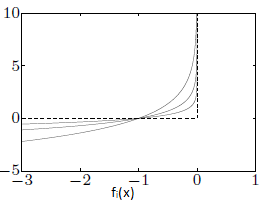
\includegraphics[width=0.9\columnwidth]{./log-barrier}
  \caption{Aproximação da função indicadora por vários valores de \textit{t}}
  \label{fig:barrier}
\end{figure}

Não sendo possível a implementação de funções não diferenciáveis, faz-se uma aproximação logarítmica, representada em (\ref{eq.log-bar}), da barreira onde é possível aplicar o método de \textit{Newton}, pelo facto de a nova formulação ser \textit{smooth}. Desta forma, escolhendo uma tolerância e um valor para \textit{t}, será possível obter uma solução sub-ótima para o problema em apenas uma iteração. No entanto, não tendo forma de escolher o valor de \textit{t} mais apropriado, utiliza-se o \textit{Barrier Method} que permite efetuar várias otimizações da função $f(z)$, a partir do parâmetro \textit{t}.
À medida que \textit{t} tende para um valor elevado, espera-se que o valor sub ótimo, $x^\ast(t)$, se aproxime do valor ideal, $x^\ast$. Quando \textit{t} tende para infinito espera-se que $x^\ast(t)$ tenda para $x^\ast$, e que este valor seja a solução do nosso problema. As soluções de cada iteração estão situadas ao longo do \textit{central path} que corresponde ao conjunto de soluções $x^\ast(t)$. Estas soluções são caracterizadas pelas \textit{KKT Conditions} e são, usualmente, denominadas de \textit{central points}. O \textit{Barrier Method} é iterativo, pelo que, a cada iteração, chamada \textit{outer iteration}, é computada uma solução sub ótima, esta solução é depois utilizada com ponto inicial de próxima iteração, estende-se esta computação até que o \textit{stopping criterion} seja verificado. A cada iteração o valor de \textit{t} é aumentado por um fator $\mu$, este fator é denominado de \textit{barrier parameter} e controla o valor que a \textit{log barrier} toma. O \textit{stopping criterion} é obtido através do \textit{duality gap} e é dado por $f(x^\ast(t))-f^\ast \leq m/t$, em que m é o número de \textit{contraints} existentes no problema e $f(x^\ast(t))-f^\ast$ o \textit{duality gap}, ou seja, a diferença entre a solução sub ótima e a ótima, e irá ser substituído por $\epsilon$, ou nível de precisão, como se observa na descrição do método. Como referido acima, espera-se que, quando \textit{t} tenda para infinito, $f(x^\ast(t))-f^\ast$ tenda para zero.

A implementação do algoritmo \textit{Barrier Method}\cite{BARRIER} seguirá o seguinte pseudo-código:

\begin{algorithmic}[1]
\renewcommand{\algorithmicrequire}{\textbf{Input:}}
\REQUIRE $x \textit{ strictly feasible}, t > 0, \mu > 1, \epsilon > 0$

\STATE obtenção de $x^* (t)$ pela minimização de $t f_0 + \phi$
\STATE Atualização de $x:=x^* (t)$
\STATE \textbf{If}($m/t < \epsilon$) \textbf{then} Stop
\STATE Incremento de $t$. $t:=\mu t$.
\end{algorithmic}

No \textit{Barrier Method} a escolha dos parâmetros \textit{t} e $\mu$ é de grande importância. Caso $\mu$ seja muito pequeno irão ser necessárias muitas \textit{outer iterations}, visto que o aumento de \textit{t} será reduzido, por outro lado, caso $\mu$ seja muito elevado, irão ser necessárias muitas iterações do método de \textit{Newton}, já que as soluções sub ótimas de iterações consecutivas irão estar muito afastadas entre si. Quanto ao valor de \textit{t} inicial, se este for muito pequeno, irão ser também necessárias muitas \textit{outer iterations}, a adaptação à função indicadora será feita lentamente, caso \textit{t} inicial seja muito elevado, a primeira iteração do método de \textit{Newton} (\textit{first centering step}) irá requerir muitas iterações para calcular $x^\ast$ inicial.

\begin{figure}[htp]
\captionsetup{font=scriptsize}  
  \centering
  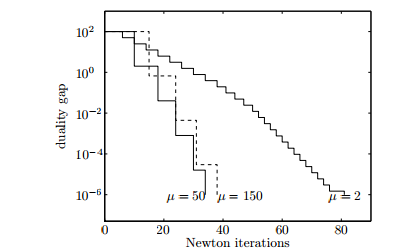
\includegraphics[width=0.9\columnwidth]{./iterations_dua_gap}
  \caption{Número de iterações de \textit{Newton} em relação a $\mu$}
  \label{fig:gamma}
\end{figure}

Na figura \ref{fig:gamma} está representada a relação entre $\mu$ e o número de iterações do método de \textit{Newton} e, como se pode observar existe um grande discrepância no número de iterações entre $\mu$ igual 2 e a 50. Pelo que o $\mu$ sugerido por \textit{Boyd e Vandenberghe} está entre os valores 10 e 50.

Neste algoritmo, faz-se no primeiro passo a minimização com recurso ao método de \textit{Newton}, sendo a função utilizada a apresentada na equação (\ref{eq.Newton}),

\begin{equation}
\label{eq.Newton}
f(z) = t f_0 (z) + \phi (z)
\end{equation}

onde

\begin{equation}
f_0 (z) = -\mu^\top (D z + b) + \gamma (D z + b)^\top \Sigma (D z + b)
\end{equation}

e

\begin{equation}
\phi = -\sum_{i=1}^{m} log(-f_i(x))
\end{equation}

O termo $\phi$ evita que a minimização com o método de Newton vá para soluções não permitidas, uma vez que a função de otimização assume o valor infinito (\textit{penalty}), obrigando o método de \textit{Newton} a calcular outro \textit{step} para encontrar uma solução viável.

Para a aplicação do método de \textit{Newton}, é ainda necessário o cálculo do gradiente e da hessiana da função $f (z)$. Como tal, o gradiente é obtido da seguinte forma:

\begin{equation}
\nabla f(z) = t (\nabla f_0(z))^\top + \nabla \phi (z)
\end{equation}

onde

\begin{equation}
\nabla f_0 (z) = -\mu^\top D + \gamma (D z + b)^\top 2 \Sigma D  
\end{equation}

e

\begin{equation}
\nabla \phi (z) = \sum_{i=1}^{m} \frac{1}{-f_i (z)} \nabla f_i (z) 
\end{equation}

A expressão da hessiana será obtida de forma idêntica pelas equações (\ref{eq.hess}), (\ref{eq.hesss}) e (\ref{eq.hessss}).

\begin{equation}
\label{eq.hess}
\nabla^2 f(z) = t (\nabla^2 f_0(z))^\top + \nabla^2 \phi (z)
\end{equation}

\begin{equation}
\label{eq.hesss}
\nabla^2 f_0 (z) = \gamma 2 (D^\top \Sigma D) 
\end{equation}

\begin{equation}
\label{eq.hessss}
\nabla^2 \phi (z) = \sum_{i=1}^{m} \frac{1}{-f_i^2 (z)} \nabla f_i (z) (\nabla f_i (z))^\top
\end{equation}

Por último, o \textit{Barrier Method} converge num número finito de iterações pelo indicado pelo ponto três do algoritmo. O número de \textit{centering steps} requerido ao \textit{Barrier Method} para atingir um nível de precisão $\epsilon$ são:

\begin{equation}
\label{steps}
\frac{log(\frac{m}{t^{(0)}\epsilon})}{log(\mu)} + 1
\end{equation}

\section{Resultados Numéricos}
\label{sec:numerical-results}

How does it really work in practice? Provide simulated performance
metrics. If possible, compare with other well-known methods.

Nas figuras que irão ser expostas tem-se a verde os resultados do \textit{Barrier Method} e a vermelho do \textit{CVX}, tanto os retornos como os riscos dos \textit{assets} são iguais para ambos os programas.
Para verificar o correto funcionamento de ambos os programas realizaram-se testes em que os resultados podem ser facilmente previstos, tais como:

\begin{itemize}
\item Igualar $\gamma$ a zero, ou seja, caso o utilizador não tenha quaisquer preocupações com o risco associado a cada investimento. Espera-se, portanto, que o portfólio obtido seja investir todo o capital no \textit{asset} com maior retorno, independentemente do risco.
\begin{figure}[htp]
\captionsetup{font=scriptsize}  
  \centering
  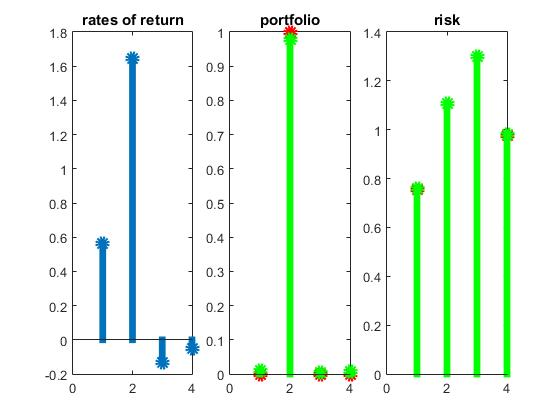
\includegraphics[width=0.9\columnwidth]{./gama_0}
  \caption{Portfólio com $\gamma$ igual a 0}
  \label{fig:caso1}
\end{figure}

Na figura \ref{fig:caso1} observa-se que, de facto, o capital foi investido no \textit{asset} de maior retorno. Existem pequenas diferenças entre o portfólio apresentado pelos dois programas, pelo que se pode observar que no resultado do \textit{CVX} o investimento é total no \textit{asset} de maior retorno, enquanto que no resultado do \textit{Barrier Method} existem pequenas quantias investidas pelos outros \textit{assets}.
\vskip 4mm

\item Igualar $\gamma$ a 100 (100 é um valor arbitrário), pretende-se ilustrar uma aversão ao risco muito elevada por parte do utilizador. Espera-se um portfólio bastante conservador, ou seja, que seja investido capital apenas no(s) \textit{asset(s)} com menor risco associado. Quando $\gamma$ tende para infinito, o portfólio será investido somente nos \textit{assets} com menor risco associado, ao contrário do caso em que $\gamma$ é igual a 100, onde existem pequenos investimentos nos outros \textit{assets}.

\begin{figure}[htp]
\captionsetup{font=scriptsize}  
  \centering
  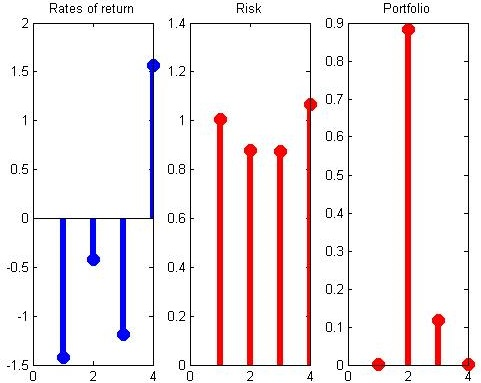
\includegraphics[width=0.9\columnwidth]{./gama_100}
  \caption{Portfólio com $\gamma$ igual a 100 e alguns retornos negativos}
  \label{fig:caso2.1}
\end{figure}

Na figura \ref{fig:caso2.1} a solução dada por ambos os programas é em tudo semelhante, note-se que, apesar das \textit{rates of return} dos \textit{assets} de menor risco serem negativas, a aversão ao risco do utilizador irá gerar um portfólio em que a importância dada ao risco é bastante superior à dos retornos. A divisão do portfólio pelos dois \textit{assets} de menor risco é a esperada, ambos os programas \: escolheram investir mais capital no \textit{asset} com maior retorno.


\begin{figure}[htp]
\captionsetup{font=scriptsize}  
  \centering
  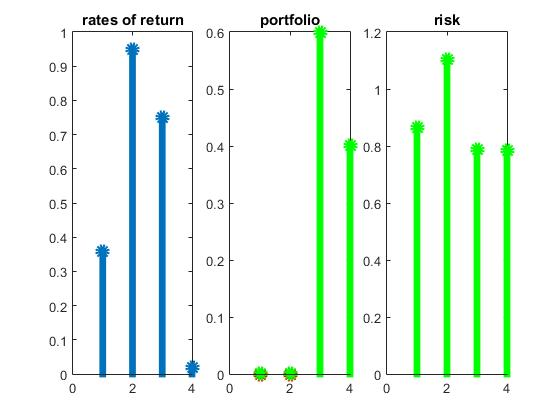
\includegraphics[width=0.9\columnwidth]{./gama_100_positivos}
  \caption{Portfólio com $\gamma$ igual a 100 e retornos positivos}
  \label{fig:caso2.2}
\end{figure}

No caso da figura \ref{fig:caso2.2}, o portfólio segue o mesmo padrão da figura \ref{fig:caso2.1}, aposta-se o capital nos \textit{assets} de menor risco e entre eles, investe-se a grande parte no \textit{asset} que apresenta maior retorno.
\vskip 4mm
\item Igualar todos o \textit{returns} e riscos de todos os \textit{assets}. O portfólio deverá dividir o capital igualmente por todos os \textit{assets}.

\begin{figure}[htp]
\captionsetup{font=scriptsize}  
  \centering
  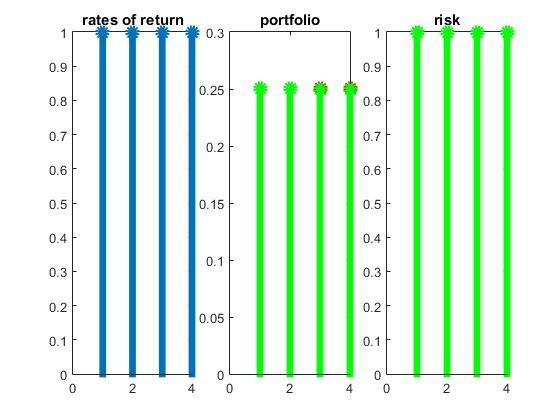
\includegraphics[width=0.9\columnwidth]{./miu_igual}
  \caption{Portfólio com riscos e retornos iguais para todos os \textit{assets}}
  \label{fig:caso3}
\end{figure}
\vskip 4mm
Na figura \ref{fig:caso3} os resultados do portfólio refletem o esperado, visto que ambos os programas repartiram igualmente o capital por todos os \textit{assets}.
\vskip 4mm
\item Igualar apenas os \textit{returns} de todos os \textit{assets}. O portfólio deverá investir a grande parte do seu capital no \textit{asset} de menor risco. Quando se aumenta $\gamma$ nesta situação é esperado que a quantidade investida no \textit{asset} de menor risco aumente.

\begin{figure}[htp]
\captionsetup{font=scriptsize}  
  \centering
  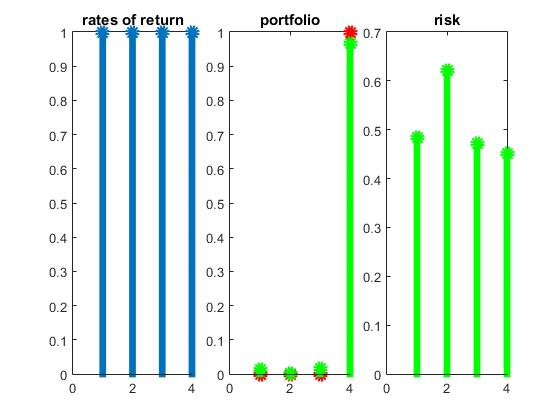
\includegraphics[width=0.9\columnwidth]{./miu_igual_risco_diferente}
  \caption{Portfólio com retornos iguais para todos os \textit{assets}}
  \label{fig:caso4}
\end{figure}

No caso enunciado acima, a solução de portfólio ótima é intuitiva, os programas deverão investir todo o capital no \textit{asset} de menor risco, visto que todos retornam o mesmo valor do investimento inicial. É isto que se comprova na figura \ref{fig:caso4}.

\end{itemize} 


The commentary of the plots should not just repeat the graphically
obvious such as "the solution is different from the original signal",
but explain, for example, how this difference relates to quick changes
on the signal. Is the solution too slow to follow the signal
variations? What is the magnitude of the error?

\begin{figure}[htp]
  \centering
  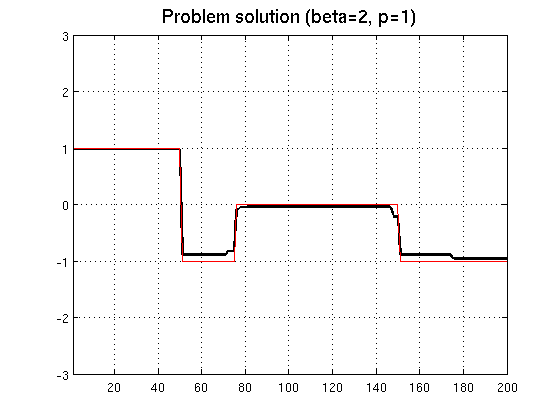
\includegraphics[width=0.9\columnwidth]{./solution1}
  \caption{Solution for the L1 norm cost function.}
  \label{fig:solution-l1}
\end{figure}

You might also want to vary the problem's parameters and see how the
solution evolves. Don't forget to explain why is the choice of
parameters in the solution depicted in Figure~\ref{fig:solution-l1}
better than the others.

Figures should be chosen wisely. You can never lay out the whole
parameter space, so provide insight into which parameters are
significant over what range and which ones are less important.



\section{Conclusões}
\label{sec:conclusion}

In general a short summarizing paragraph will be sufficient. It should
not simply repeat material from the Abstract or Introduction. In some
cases it's possible to now make the original claims more concrete,
\textit{e.g.}, by referring to quantitative results.


\begin{thebibliography}{9}

\bibitem{CVX}
  [CVX15] \texttt{http://cvxr.com/cvx}, Junho 2015
  
\bibitem{BARRIER}
  [BV\_CVXSLIDES] \texttt{https://web.stanford.edu/boyd/cvxbook/ bv\_cvxslides.pdf}


\end{thebibliography}

\end{document}
This is never printed 